\documentclass[
	a4paper 			% paper size
	,12pt				% font size
	,titlepage
	,twoside
	,listof=totoc 		% adds list of figures and tables to the table of contents
	,bibliography=totoc	% adds the references to the table of contents
	,numbers=noenddot 	% avoid some irritating dots at the end of figure numbers when using appendix
	]{scrreprt}




\usepackage{ifthen}

% ---------------------------------------------------------------
% page layout
% ---------------------------------------------------------------
\usepackage{geometry}
\geometry{twoside,inner=2.5cm, top=2cm, outer=2cm, bottom = 2cm, includefoot, includehead}

% Caption design
\usepackage[bf,sf,nooneline]{caption} % see caption manual for more information
\captionsetup{format=plain}

% ---------------------------------------------------------------
% figures
% ---------------------------------------------------------------
\usepackage{float} 					% force figures to location with [H]
\usepackage[figuresright]{rotating} % rotation of figures
\usepackage{subfigure}				% stack and arange figures
\usepackage{graphics} 				% you now may use jpg
\usepackage{eso-pic}				% include images covering the whole page (see title page)
\usepackage{overpic}				% you can use this package to write over your figure, see manual
\setlength{\subfigcapmargin}{0.5em} % see subfigure package - spacing between labels captions of subfigures

% ---------------------------------------------------------------
% tikz, pstricks style drawing
% ---------------------------------------------------------------
\usepackage{tikz,pgfplots,pgfkeys}	% for drawings (similar to pstricks and Co.)
\usepackage{psfrag} % Only for LaTeX
% ---------------------------------------------------------------
% type face
% ---------------------------------------------------------------
\usepackage[T1]{fontenc}    %% 
% \usepackage[latin1]{inputenc} 
\usepackage[utf8]{inputenc} %%% use utf8x encoding instead latin1

% RUB fonts, if installed
%\renewcommand{\sfdefault}{rubflama}
%\renewcommand{\rmdefault}{rubscala}

% if not you can use these fonts.
% sans serif
\usepackage{helvet}
% serif
\usepackage{lmodern}

\usepackage{pdfpages}

% ---------------------------------------------------------------
% symboles und math
% ---------------------------------------------------------------
\usepackage{amsmath} % math envoirment.
\usepackage{amssymb} 	% more symbols for writing
\usepackage{amsfonts}
\usepackage{fixmath}	% fixes some errors in amsmath
\usepackage{upgreek}
% ---------------------------------------------------------------
% language
% ---------------------------------------------------------------
\usepackage[
%	german,		% Alte deutsche Rechtschreibung
%	ngerman,	% Neue deutsche Rechtschreibung
	english,	% english
%	french,		% francais
]{babel}

% ---------------------------------------------------------------
% footnotes
% ---------------------------------------------------------------
\usepackage{chngcntr} 
\counterwithout{footnote}{chapter} 	% avoids the footnote counter reset after each chapter

% ---------------------------------------------------------------
% literature list
% ---------------------------------------------------------------
% Bibliography using bibtex, include to your document with  \bibliography{bibtex-datei}
% some examples for different bibtex-styles
% \bibliographystyle{plain}
%\bibliographystyle{acm}
\bibliographystyle{plaindin}
%\bibliographystyle{is-abbrv}

% ---------------------------------------------------------------
% Hyperref
% ---------------------------------------------------------------
%% colored links for pdf
%\definecolor{pdfurlcolor}{rgb}{0,0,0.6}
%\definecolor{pdffilecolor}{rgb}{0.7,0,0}
%\definecolor{pdflinkcolor}{rgb}{0,0,0.6}
%\definecolor{pdfcitecolor}{rgb}{0,0,0.6}

% link color for print, black
\definecolor{pdfurlcolor}{rgb}{0,0,0}
\definecolor{pdffilecolor}{rgb}{0,0,0}
\definecolor{pdflinkcolor}{rgb}{0,0,0}
\definecolor{pdfcitecolor}{rgb}{0,0,0}

\usepackage[
   % link color
   colorlinks=true,         % links are colored, not with boxes
   urlcolor=pdfurlcolor,    % \href{...}{...} external (URL)
   filecolor=pdffilecolor,  % \href{...} local file
   linkcolor=pdflinkcolor,  % \ref{...} and \pageref{...}
   citecolor=pdfcitecolor,  % \cite{...}
   % Links
   breaklinks,              % links work with line breaks
   bookmarksnumbered=true,  % enumerate pdf-bookmarks
   bookmarksopen=true, 		% bookmark-view: all subdirectories are open
]{hyperref}

% pdf information
\hypersetup{pdftitle={PDF-LaTeX Vorlage}}


\usetikzlibrary{shapes.multipart} % For rounded rectangles

% Define a new command for including rounded images
\newcommand{\roundedincludegraphics}[2][]{%
    \tikz\node[inner sep=0, rounded corners, outer sep=0] {\includegraphics[#1]{#2}};%
}

% ---------------------------------------------------------------
% head and foot
% ---------------------------------------------------------------
\usepackage[headsepline=.4pt]{scrlayer-scrpage}	% package for headings
\pagestyle{scrheadings} % define the default page-style for your document
% \setheadsepline{.4pt}	% underline head
% \usepackage[headsepline=.4pt]{scrlayer-scrpage}

\automark[section]{chapter} % defines leftmark and rightmark: \automark[<rightmark>]{<leftmark>}
\lehead{\leftmark} 		% left side, even page number: chapter
\rohead{\rightmark} 	% right side, odd page number: section
\ofoot{\pagemark} 		% page number


% ---------------------------------------------------------------
% misc.
% ---------------------------------------------------------------

% TODONOTES, generates a list of todos, placeholder for figures etc.
% useful package for larger documents. Just have a look at the manual.
\usepackage[
%	disable,
	shadow,colorinlistoftodos,color=green!40
	]{todonotes}


% DEFINE RUB-COLORS
% you can use the RUB colors in Matlab, too. Look at sheldon/user-public/aschasse/RUB_colors/createRubColorset.m
\usepackage{calc}
\definecolor{RUB_blue_0}{RGB}{0,53,96}
\definecolor{RUB_blue_1}{RGB}{23,82,125}
\definecolor{RUB_blue_2}{RGB}{80,117,155}
\definecolor{RUB_blue_3}{RGB}{136,157,188}
\definecolor{RUB_blue_4}{RGB}{193,203,221}

\definecolor{RUB_green_0}{RGB}{148,193,27}
\definecolor{RUB_green_1}{RGB}{174,205,82}
\definecolor{RUB_green_2}{RGB}{196,218,131}
\definecolor{RUB_green_3}{RGB}{217,230,176}
\definecolor{RUB_green_4}{RGB}{236,243,218}

\definecolor{RUB_gray_0}{RGB}{221,221,221}
\definecolor{RUB_gray_1}{RGB}{229,229,229}
\definecolor{RUB_gray_2}{RGB}{237,237,237}
\definecolor{RUB_gray_3}{RGB}{245,245,245}

\definecolor{RUB_orange_0}{RGB}{228,136,65}
\definecolor{RUB_orange_1}{RGB}{232,154,84}
\definecolor{RUB_orange_2}{RGB}{239,179,113}
\definecolor{RUB_orange_3}{RGB}{243,188,132}
\definecolor{RUB_orange_4}{RGB}{250,206,167}

\definecolor{RUB_red_0}{RGB}{198,77,50}
\definecolor{RUB_red_1}{RGB}{219,103,78}
\definecolor{RUB_red_2}{RGB}{235,134,111}
\definecolor{RUB_red_3}{RGB}{248,157,143}
\definecolor{RUB_red_4}{RGB}{252,189,179}

% ---------------------------------------------------------------
% own commands
% ---------------------------------------------------------------
% e.g.
\newcommand{\EW}[1]{\text{E}\left\lbrace #1 \right\rbrace } % Expectation


%%% Own new Commands %%%% 
\newcommand{\AUTHOR}{Ravi Rahul Kumar Shah}
\newcommand{\SUPERVISOR}{M. Sc. Luca Becker}
\newcommand{\PROF}{Prof. Dr.-Ing. Rainer Martin}
\newcommand{\TITLE}{Information Bottleneck Based Privacy-preserving Feature Extraction Using a Trainable Acoustic Frontend}


% ---------------------------------------------------------------
% \usepackage{glossaries}
% \usepackage[automake]{glossaries-extra}
% \preto\section{\glsresetall}
% \setabbreviationstyle[acronym]{long-short}

\usepackage[withpage]{acronym}
% \usepackage[style=numeric]{biblatex}
% \addbibresource{references.bib}

% \usetikzlibrary{shapes, arrows, positioning, shapes.geometric, fit}
\usepackage{cleveref}

\usepackage{tabularx}
\usepackage{array}
\usepackage{booktabs}
\raggedbottom

% \usetikzlibrary{shapes.geometric, arrows, positioning, fit}
% \makeglossaries
\setlength{\glslistdottedwidth}{.5\textwidth}
\newacronym{gdpr}{GDPR}{General Data Protection Regulation}
\newacronym{ccpa}{CCPA}{California Consumer Privacy Act}
\newacronym{lgpd}{LGPD}{Brazilian General Data Protection Law}
\newacronym{iot}{IoT}{Internet of Things}


\newacronym{lmbe}{LMBE}{Log Mel Band Energy}
\newacronym{pcen}{PCEN}{Per Channel Energy Normalization} 
\newacronym{mfcc}{MFCC}{Mel Frequency Cepstral Coefficients}
\newacronym{melspec}{MelSpec}{Mel Spectrogram}
\newacronym{stftspec}{STFTSpec}{STFT Spectrogram}

\newacronym{fft}{FFT}{Fast Fourier Transform}
\newacronym{dft}{DFT}{Discrete Fourier Transform}
\newacronym{stft}{STFT}{Short Time Fourier Transform}
\newacronym{zcr}{ZCR}{Zero Crossing Rate}
\newacronym{mse}{MSE}{Mean Squared Error}
\newacronym{mae}{MAE}{Mean Absolute Error}

\newacronym{ai}{AI}{Artificial Intelligence}
\newacronym{ml}{ML}{Machine Learning}
\newacronym{dl}{DL}{Deep Learning}
\newacronym{svm}{SVM}{Support Vector Machine}
\newacronym{svr}{SVR}{Support Vector Regression}
\newacronym{dnn}{DNN}{Deep Neural Network}
\newacronym{nn}{NN}{Neuronal Network}
\newacronym{ann}{ANN}{Artificial Neural Network}
\newacronym{cnn}{CNN}{Convolutional Neural Network}

\newacronym{mlp}{MLP}{Multi Layer Perceptron}
\newacronym{relu}{ReLU}{Rectified Linear Unit}
\newacronym{elu}{ELU}{Exponential Linear Unit}

\newacronym{rnn}{RNN}{Recurrent Neural Network}


\newacronym{lstm}{LSTM}{Long Short Term Memory}

\newacronym{vae}{VAE}{Variational Autoencoder}

\newacronym{sgd}{SGD}{Stochastic Gradient Descent}

\newacronym{mbgd}{MBGD}{Mini-Batch Gradient Descent}
\newacronym{gr}{GR}{Gender Recognition}
\newacronym{si}{SI}{Speaker Identification}
\newacronym{auprc}{AUPRC}{Area Under the Precision-Recall Curve}

\newacronym{adam}{ADAM}{Adaptive Moment Estimation}

\newacronym{gan}{GAN}{Generative Adversarial Network}

\newacronym{wasn}{WASN}{Wireless Acoustic Sensor Network} 

\newacronym{vib}{VIB}{Variational Information Bottleneck}
\newacronym{ust}{UST}{Urban Sound Tagging}

mutual information 
\setcounter{tocdepth}{1}

%%%%%%%%%%%%%%%%%%%%%%%%%%%%%%%%%%%%%%%%%%%%%%%%%%%%%%%%%%%%%%%
%                        BEGIN DOCUMENT                       %
%%%%%%%%%%%%%%%%%%%%%%%%%%%%%%%%%%%%%%%%%%%%%%%%%%%%%%%%%%%%%%%
\begin{document}

% ---------------------------------------------------------------
% title page
% ---------------------------------------------------------------
\thispagestyle{empty}

\newboolean{myLanguageIsEnglish}
\setboolean{myLanguageIsEnglish}{true} % <--- EDIT!
\ifthenelse{\boolean{myLanguageIsEnglish}}
{
\AddToShipoutPicture*{\put(0,0){
\includegraphics[]{Template/title_background_english}}}
}{% else
\AddToShipoutPicture*{\put(0,0){
\includegraphics[]{Template/title_background_german}}}
}
\vspace*{3.5cm}
\begin{flushleft}
\Huge % for longer titles you can use other font sizes (e.g. \huge, \Large, etc.)
Bachelor Thesis \newline % Enter here the type of your work (Master-, Bachelor-, Diplom- oder Studienarbeit)
\bfseries
\textsf{\TITLE} % Enter the title of your work
\end{flushleft}
\vspace*{0.5cm}
\begin{Large}
\textbf{\AUTHOR} % This is the author
\vspace*{2cm}
\vfill
\begin{flushleft}
\ifthenelse{\boolean{myLanguageIsEnglish}}
{Advised by:\newline}
{Betreuung durch:\newline}
\SUPERVISOR \newline
\PROF 
\vspace*{1cm}
\newline
\ifthenelse{\boolean{myLanguageIsEnglish}}
{This thesis was developed between:\newline}
{Bearbeitungszeitraum:\newline}
26. Juni 2023 and 18. October 2023
\end{flushleft}
\end{Large}

% blank page after title
\cleardoublepage

% ---------------------------------------------------------------
% declaration
% ---------------------------------------------------------------
\newpage
\thispagestyle{empty}
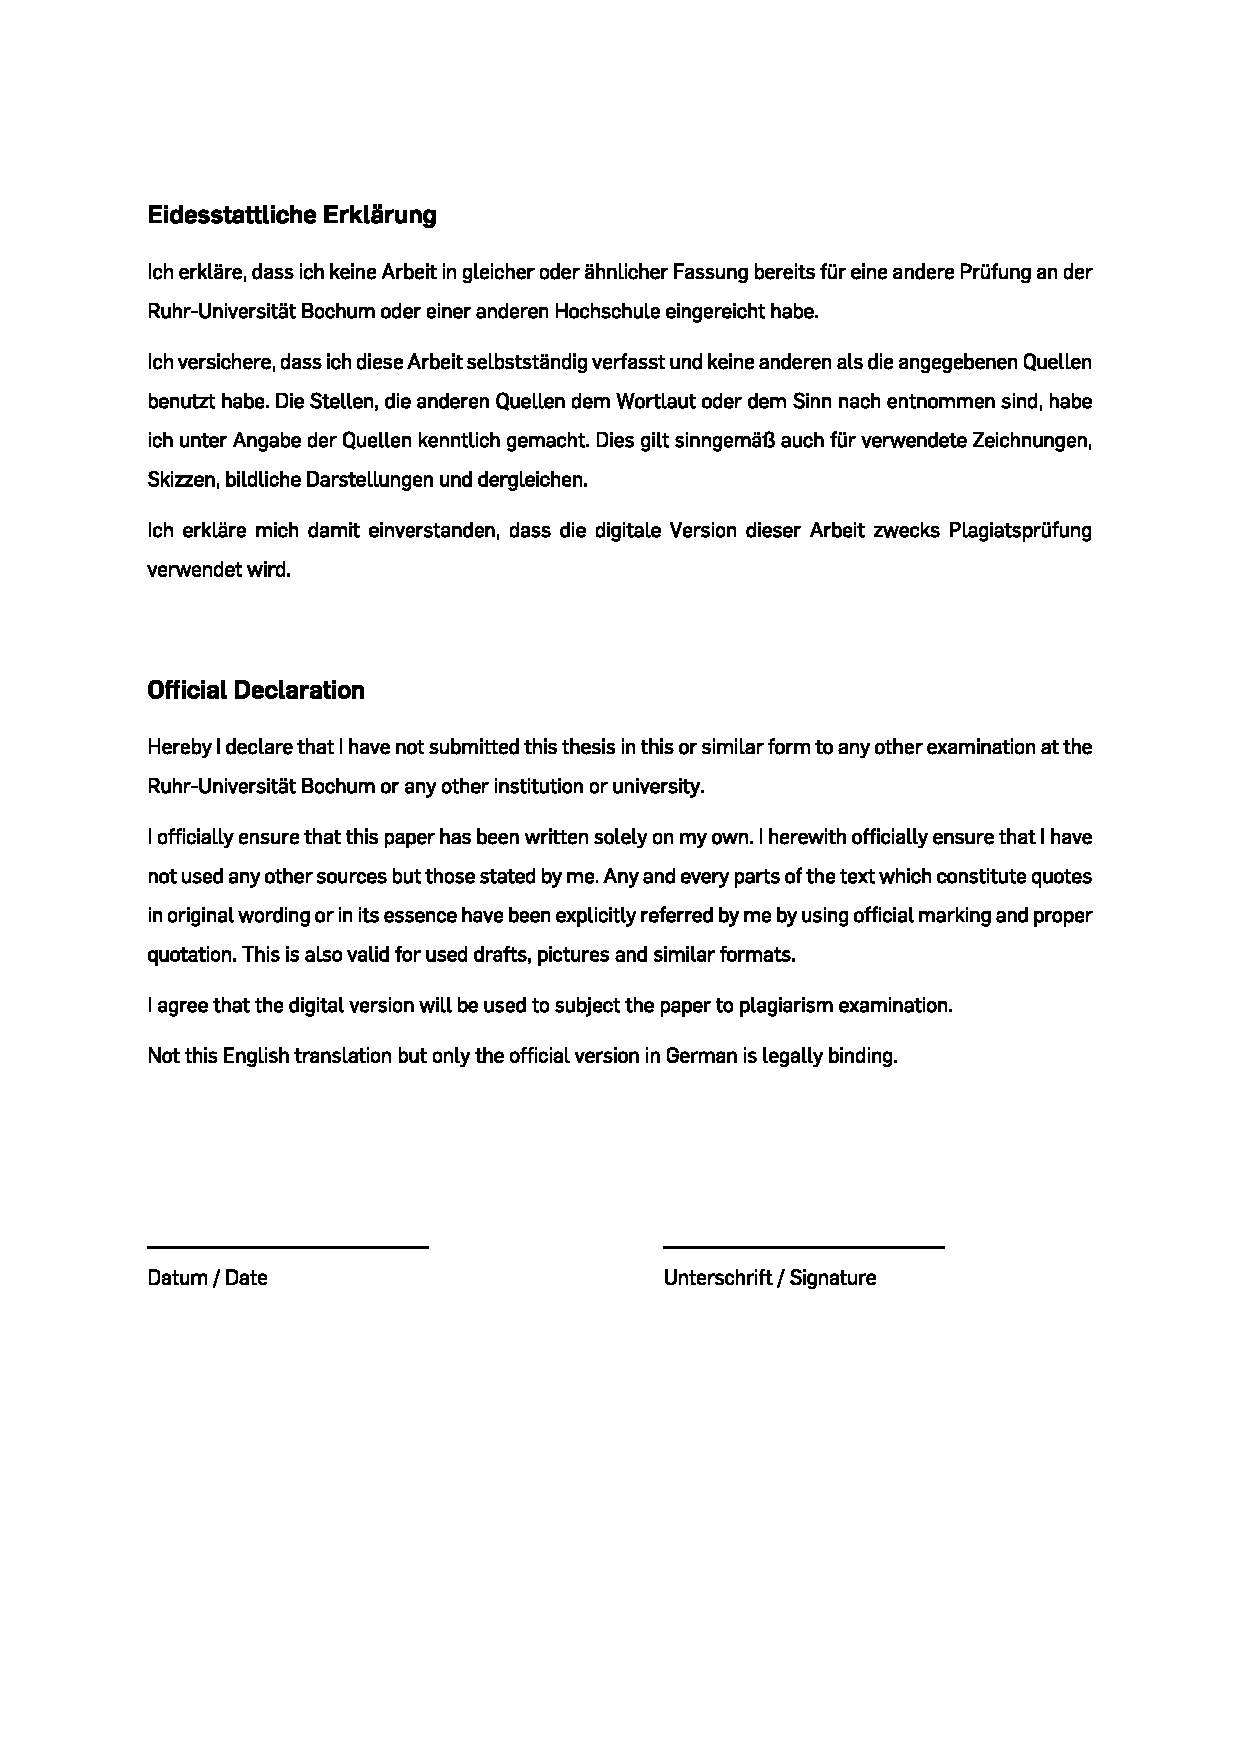
\includepdf[pages=-]{EidesstattlicheErklaerungPO13.pdf}

\cleardoublepage

% ---------------------------------------------------------------
% table of contents
% ---------------------------------------------------------------
\newpage
\tableofcontents
\renewcommand{\thepage}{\Roman{page}}
\setcounter{page}{1}

% ---------------------------------------------------------------
% list of figures
% ---------------------------------------------------------------
\newpage
\listoffigures

% ---------------------------------------------------------------
% list of tables
% ---------------------------------------------------------------
% \listoftables

% ---------------------------------------------------------------
% list of abbreviations
% ---------------------------------------------------------------
\chapter*{List of Abbreviations} \addcontentsline{toc}{chapter}{List of Abbreviations}

% \printglossary[type=\acronymtype,nonumberlist]
% \begin{acronym}%[LINUX]
    \acro{GDPR}{General Data Protection Regulation}
    \acro{CCPA}{California Consumer Privacy Act}
    \acro{LGPD}{Brazilian General Data Protection Law}
    \acro{IOT}{Internet of Things}
    \acro{WASN}{Wireless Acoustic Sensor Network} 
    
    \acro{LMBE}{Log Mel Band Energy}
    \acro{PCEN}{Per Channel Energy Normalization} 
    \acro{MFCC}{Mel Frequency Cepstral Coefficients}

    
    \acro{FFT}{Fast Fourier Transform}
    \acro{DFT}{Discrete Fourier Transform}
    \acro{STFT}{Short Time Fourier Transform}
    \acro{MSE}{Mean Squared Error}
    \acro{RNN}{Recurrent Neural Network}
    \acro{LSTM}{Long Short Term Memory}
    \acro{VAE}{Variational Autoencoder}
    
    \acro{AI}{Artificial Intelligence}
    \acro{ML}{Machine Learning}
    \acro{DL}{Deep Learning}
    \acro{SVM}{Support Vector Machine}
    \acro{SVR}{Support Vector Regression}
    \acro{DNN}{Deep Neural Network}
    \acro{NN}{Neuronal Network}
    \acro{MLP}{Multi Layer Perceptron}
    \acro{ANN}{Artificial Neural Network}
    \acro{RELU}{Rectified Linear Unit}
    \acro{ANN}{Artificial Neural Network}
    \acro{CNN}{Convolutional Neural Network}
    \acro{GAN}{Generative Adversarial Network}
    \acro{VIB}{Variational Information Bottleneck}
    
    
    \acro{SGD}{Stochastic Gradient Descent}
    \acro{MBGD}{Mini-Batch Gradient Descent}
    \acro{GR}{Gender Recognition}
    \acro{SI}{Speaker Identification}
    \acro{UST}{Urban Sound Tagging}
    \acro{AUPRC}{Area Under the Precision-Recall Curve}
    
    % \acro{ADAM}{Adaptive Moment Estimation}

    


    
\end{acronym}
% ---------------------------------------------------------------
% glossary, german: Nomenklatur, bzw. Liste der Verwendeten Formelzeichen
% ---------------------------------------------------------------
% \chapter*{Glossary} \addcontentsline{toc}{chapter}{Glossary}

% ---------------------------------------------------------------
% abstract
% ---------------------------------------------------------------
% \chapter*{Abstract} \addcontentsline{toc}{chapter}{Abstract}

% to make sure, that the first chapter starts on a right hand page.
\cleardoublepage

% ---------------------------------------------------------------
% Introduction
% ---------------------------------------------------------------
\newpage
% set page numbering to arabic, reset page counter
\renewcommand{\thepage}{\arabic{page}}
\setcounter{page}{1}
\chapter{Introduction}

Over the past decade, the proliferation of smart home and Internet of Things (IoT) devices has considerably enhanced the quality of our daily lives. However, these technological advancements come at a hidden cost. With the advancements in complex machine learning algorithms, there have been growing concerns about the sensitive data collected by big tech companies and the potential misuse of this information.\\
Speech signals encapsulate a wealth of information and can reveal a multitude of characteristics such as accent, pitch, speed, gender, health status, and the emotional state of the speaker. By analyzing the content of speech like tone, bass, timbre, articulation, rhythm, stress patterns, and phonetic nuances over time, one can discern not only the overt message being conveyed but also subtle cues that hint at the speaker's background, upbringing, and current state of mind. These cues, when interpreted correctly, can provide insights into shopping preferences, linguistic habits, social interactions, and behavioral patterns. Using advanced machine learning methodologies, a comprehensive profile of an individual user can be derived, particularly when distinct speaker identification is achievable.
In reaction to growing concerns, a myriad of legal frameworks and standards have been instituted globally. Prominent among these are the European Union’s General Data Protection Regulation (GDPR) \cite{gdpr}, the California Consumer Privacy Act (CCPA) \cite{ccpa}, and Brazil’s General Personal Data Protection Law (LGPD) \cite{lgpd}. These regulations mandate corporations to integrate \textit{privacy-by-design} principles during the development of signal processing systems. Consequently,  these have amplified the urgency and significance of research in the arena of privacy-preserving signal processing.\\



\textit{Utility} represents the enhanced capabilities and service quality offered by modern speech command services provided by corporations. However, the pursuit of this \textit{utility} inherently involves a trade-off: the risk of data exposure, thereby compromising \textit{privacy}. \textit{Utility} emphasizes the functionality and efficiency of a service, aiming to maximize user benefit and experience, while \textit{privacy} prioritizes the protection of personal information to ensure that users' data remains confidential and secure. While \textit{utility} seeks optimization through data analysis, \textit{privacy} cautions against potential overreach and misuse. Balancing \textit{utility} and \textit{privacy} is a challenge, as it aims to maximize service efficiency while safeguarding user data.\\

The privacy enhancement approach in this project incorporates the use of a feature extraction model, transmitting only the essential features from the raw data to the server, thereby minimizing mutual information. This method is inspired by the paper \cite{nelus}, aiming to optimize accuracy in gender discrimination (\textit{utility}) while ensuring the results for speaker identification remain non-distinctive to maintain \textit{privacy}. This approach draws inspiration from the concept of the \textit{Variational Information Bottleneck} (VIB) \cite{alemi2017deep}, which is motivated by the \textit{Information Bottleneck} (IB) principle \cite{tishby2000information}. This principle aims to retain only the most relevant information for a task, thereby reducing the risk of exposing unnecessary data. The VIB method incorporates elements of the \textit{variational autoencoder}, a type of neural network(NN) that can generate new, similar data based on the training set. This technique encodes compact data representations and employs a \textit{re-parametrization} method \cite{kingma2013auto}, introducing variability and allowing for stochastic sampling during backpropagation. This helps optimize the balance between \textit{utility} and \textit{privacy} by ensuring that the model does not overfit to sensitive information.\\


In this project, we deploy a deep neural network(DNN)-based, privacy-aware feature extraction technique for gender recognition(GR) and speaker identification(SI), as detailed in the referenced paper \cite{nelus}. The primary goal is to balance the trade-off between GR and SI, thereby mitigating potential data exposure risks by minimizing the amount of data transferred over the channel. Our investigation into this scenario aims to enhance the classifier's GR capabilities while simultaneously restricting access to precise speaker identity information.

The aim of this work is to examine the effectiveness of the trainable acoustic frontend, Per Channel Energy Normalization (PCEN), in GR vs SI tasks. To evaluate this, we compared the performance of Per Channel Energy Normalization(PCEN) with that of Log Mel Band Energy (LMBE) as a feature extractor. We evaluated the performance of PCEN with both trainable and non-trainable parameters. We utilized the \textit{Librispeech} dataset for our experiment and extracted high-level features by training the GR trust model. Next, applying the VIB principle, we established a probabilistic mapping between the input data and a compact latent space through the \textit{re-parametrization trick}, as discussed in \cref{sec:rpTrick}. By leveraging the VIB principle and gradually increasing the budget scaling factor \( \beta \), our goal is to identify a \( \beta \) at which the features compress in such a way that GR remains achievable, but SI becomes challenging. Furthermore, we investigated the accuracy of the SI by training the high-level feature extractor, referred to as the Trust model, using the \textit{Sonyc UST} dataset.


Before transmitting information to the server side, a scheme can be applied at the node level that employs deep neural network (DNN)-based feature extraction. We utilize a privacy-centric variational information feature extraction technique that deliberately produces lossy results, anchoring on Mutual Information (MI) minimization. Our analysis focuses on its impact on the delicate balance between GR accuracy (\textit{utility}) and SI (\textit{privacy}). Striking a balance between these two elements is crucial; optimizing one often compromises the other. We examine the loss function and the budget scaling factor \( \beta  \), which influences the trade-off between \textit{utility} and \textit{privacy}, for our proposed model. Experimental results have demonstrated that our method substantially mitigates the associated privacy risks without causing significant degradation in \textit{utility}. Impressively, these outcomes are also consistent with speech sources not previously observed. In the context of wireless acoustic sensor networks (WASNs), implementing node-level feature extraction is especially beneficial as it offers the potential to decrease bandwidth consumption, distribute computational load across the network, and hence enhance \textit{privacy} by incorporating aggregation techniques.

\pagebreak

The structure of the thesis is organized as follows:

\begin{itemize}
    \item \textbf{Chapter 2: Feature Extraction} provides an overview of various techniques, emphasizing the detailed discussion on Log Mel Band Energy (LMBE) and Per Channel Energy Normalization (PCEN).
    
    \item \textbf{Chapter 3: Fundamentals of Deep Learning Networks} delves into the core concepts of DNN, covering topics such as activation functions, optimization methods, Convolutional Neural Networks (CNN), and the training processes of DNNs.
    
    \item \textbf{Chapter 4: Privacy-preserving Feature Extraction} explores methodologies and principles for preserving privacy in feature extraction, including discussions on the Variational Autoencoders (VAE), Variational Information Bottleneck(VIB) principle and the reparametrization trick.
    
    \item \textbf{Chapter 5: Experimental Setup and Results} details the experimental framework for both the \textit{Librispeech} and \textit{SONYC UST} datasets and presents the findings obtained from the experiments.
\end{itemize}


% \include{kap2/}
% \include{kap3/}
% \include{kap4/}
% \include{kap5/}



\cleardoublepage




% \section{References}

\cleardoublepage

% ---------------------------------------------------------------
% conclusion
% ---------------------------------------------------------------
\chapter*{Conclusions} \addcontentsline{toc}{chapter}{Conclusions}


\section*{Future Work}

\begin{itemize}
    \item \textbf{Exploration of PCEN Parameters:} A promising avenue for future research lies in the exploration of specific parameters within PCEN. Fine-tuning these parameters could potentially enhance the performance difference between the GR and SI tasks, ensuring optimal privacy preservation.
    \item \textbf{Modifying PCEN for higher dynamic range:} One potential direction for enhancement is to modify PCEN to achieve a higher dynamic range. This could address the observed limitations of PCEN in terms of information loss and concurrent performance degradation.
    \item \textbf{Evaluation on Diverse Datasets:} To ascertain the generalizability of our findings, it would be beneficial to test them on a variety of datasets. This approach would offer a more comprehensive understanding of the strengths and limitations of both PCEN and LMBE in different contexts.
    \item \textbf{Exploring MobileNetV2 for SONYC UST Dataset}: In future endeavors, it would be worthwhile to investigate the application of the \textit{MobileNetV2} architecture for the SONYC UST dataset. Given MobileNetV2's efficiency in terms of computational resources and its adaptability to various tasks, it presents a promising avenue for enhancing classification performance. The compact nature of MobileNetV2 might offer a balance between accuracy and computational efficiency, making it particularly suitable for real-time or on-device applications related to the SONYC UST dataset.
\end{itemize}


% ---------------------------------------------------------------
% literature list -> edit references.bib to enter bibtex-code
% ---------------------------------------------------------------
% \bibliography{references}
% \pagebreak
% \printbibliography
\bibliography{references.bib}
% ---------------------------------------------------------------
% list of todos -> todonotes package
% ---------------------------------------------------------------
% \listoftodos

%%%%%%%%%%%%%%%%%%%%%%%%%%%%%%%%%%%%%%%%%%%%%%%%%%%%%%%%%%%%%%%
%                         END DOCUMENT                        %
%%%%%%%%%%%%%%%%%%%%%%%%%%%%%%%%%%%%%%%%%%%%%%%%%%%%%%%%%%%%%%%
 \raggedbottom
\end{document}